% LTeX: language=fr

\chapter{Implémentation de la solution}





\section{Serveur FTP}

Pour éviter qu'un utilisateur puisse télécharger un malware depuis l'extérieur par inadvertance, l'organisation du système de fichier a dû être réfléchie en profondeur. Il y a deux utilisateurs: \textit{upload} et \textit{analysis} qui ont chacun leur dossier comme vous pouvez le voir sur la figure \ref{fig:ftp-folders}. Ils ne peuvent pas exécuter la moindre commande sur le serveur, ils sont restreints à la seule utilisation du serveur FTP. En autorisant l'utilisateur upload uniquement à modifier le contenu de son dossier (il n'a même pas le droit de lire les fichiers qu'il contient), on empêche effectivement la possibilité que des malwares puissent sortir du réseau isolé.

% \begin{customquote}
% \begin{verbatim}
% /ftp/
% ├─ d rwx --- ---       analysis analysis  ./analysis/ <== analysis = tout, upload = /
% │     └─ - --- r-- --- analysis analysis  ./fichier   <== analysis = tout, upload = /
% └─ d rwx r-s ---       upload analysis    ./upload/   <== analysis = lecture, upload = tout
%       └─ - --- r-- --- upload analysis    ./fichier   <== analysis = lecture, upload = écriture
% \end{verbatim}
% \end{customquote}

\begin{figure}
    \centering
    \makebox[\textwidth]{
        \resizebox{17cm}{!}{
            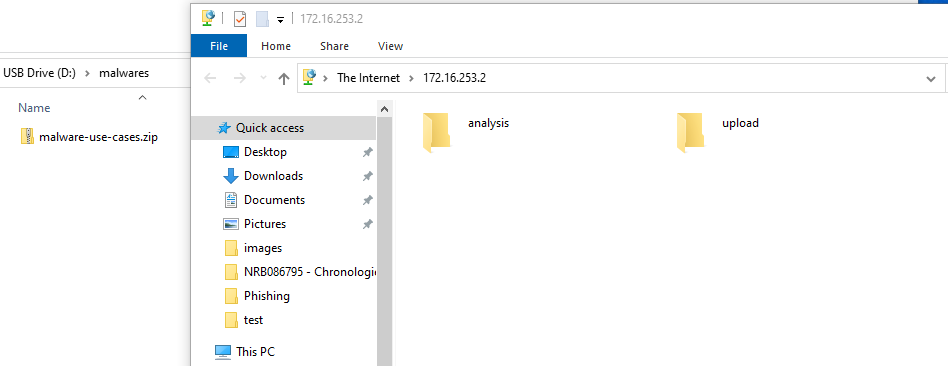
\includegraphics[width=0.95\linewidth]{images/infra-sandbox/ftp-folders.png}
        }
    }
    \caption{Structure de fichiers du serveur FTP.}
    \label{fig:ftp-folders}
\end{figure}





\section{SIFT/REMnux}

Dans cette machine virtuelle d'analyse basée sur Ubuntu qui a été installée à partir de SIFT, il faut bien sûr rajouter la distribution REMnux par-dessus, ce qui se fait facilement puisqu'il suffit de télécharger l'exécutable remnux depuis le répertoire GitHub du projet. Ensuite, il faut installer la plateforme d'analyse automatique de malware FAME et la sandbox CAPE à partir de leurs répertoires GitHub. Pour que FAME puisse communiquer correctement avec CAPE, il a fallu modifier le module FAME qui communiquait avec la sandbox Cuckoo dont CAPE est un fork, c'est-à-dire une copie modifiée.

Ensuite, comme vous pouvez le voir sur la figure \ref{fig:virt-manager}, une machine virtuelle Windows 10 imbriquée a été installée à l'intérieur de SIFT/REMnux. Cette machine imbriquée peut être réinitialisée à volonté par CAPE pour analyser des malwares dans un environnement sain. Pour éviter d'avoir du bruit parasite dans les rapports fournis par CAPE, comme une communication vers un domaine Microsoft parce que le système d'exploitation cherche si des mises à jour sont disponibles, autrement dit: pour avoir moins de faux positifs, il a fallu arrêter plusieurs services et configurer Windows pour arrêter ce genre de requêtes.

\begin{figure}[H]
    \centering
    \makebox[\textwidth]{
        \resizebox{14cm}{!}{
            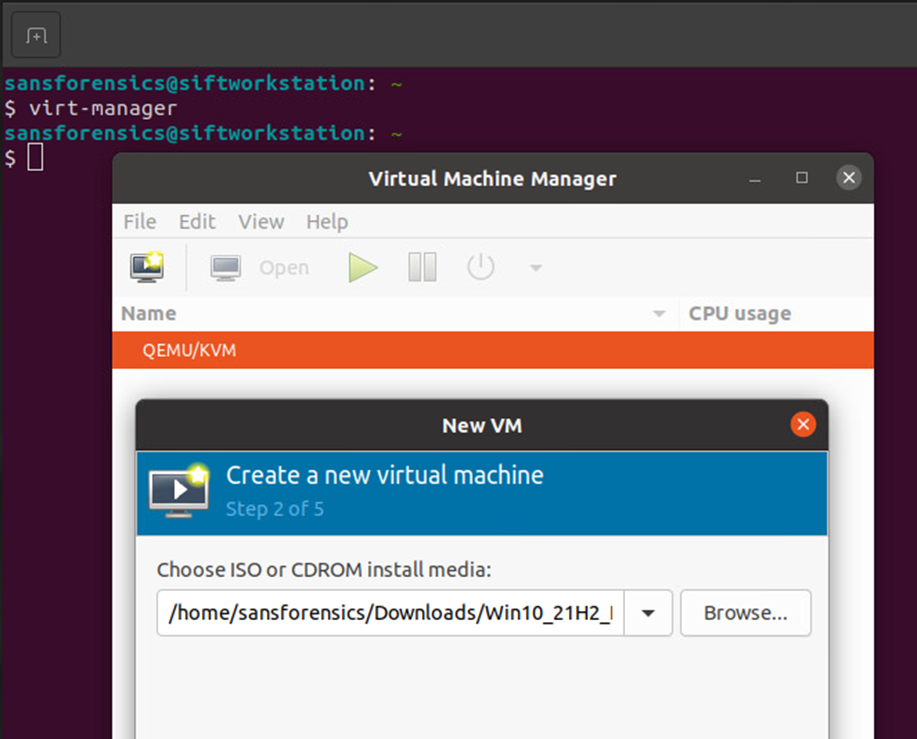
\includegraphics[width=0.95\linewidth]{images/infra-sandbox/install-virt-manager.png}
        }
    }
    \caption{Création d'une machine virtuelle Windows 10 imbriquée pour la sandbox.}
    \label{fig:virt-manager}
\end{figure}





\section{FLARE VM}

L'installation de cette machine virtuelle d'analyse basée sur Windows est très simple. Tout d'abord, on peut télécharger une machine virtuelle Windows de test fournie par Microsoft. Ensuite, il suffit de télécharger un script PowerShell sur le répertoire GitHub du projet et de l'exécuter avec des privilèges administrateurs. Ce script va apporter toutes les modifications nécessaires au système d'exploitation et installer presque tous les outils dont nous avons besoin. Il en manque seulement quelques-uns, en particulier des logiciels qui ne sont pas open source comme ArsenalImageMounter et Kape.

